\section{Experiments}

In this section, we provide empirical results on MNIST dataset to demonstrate the effectiveness of our proposed algorithms. The model we use is the LeNet [ ] CNN architecture, with 60,000 model parameters in total.

Four methods are compared in our experiments: Federated SGD (FedSGD), SketchSGD~\cite{ivkin2019communication}, FedSketch-PRIVIX (FS-PRIVIX for short) and FedSketch-HEAPRIX (FS-HEAPRIX). We implement the algorithms in Pytorch by simulating the distributed and federated environment. Note that in Algorithm~\ref{Alg:PFLHom}, FS-PRIVIX with global learning rate $\gamma=1$ is equivalent to the DiffSketch approach proposed in \cite{li2018federated}. In all experiments, we set the number of workers to $50$. For federated learning algorithms, we use different number of local updates $\tau$. For SketchedSGD which is under synchronous distributed learning framework, $\tau$ is fixed as $1$. For all methods, we tune the learning rates (both local and global, if applicable) over the log-scale and report the best results.

In each round of local update, we randomly choose half of the local devices to be active, which is more practical in real-world applications. For the data distribution on each device, we test both homogeneous and heterogeneous setting. The the first case, each device receives uniformly chosen data samples (each class has equal probability). In the later case, every device only receives samples from one or two classes among ten digits in the MNIST dataset. Since data is not distributed i.i.d. among local devices, training is expected to be harder in the heterogeneous case.

\begin{figure}[h]
	\begin{center}
		\mbox{			    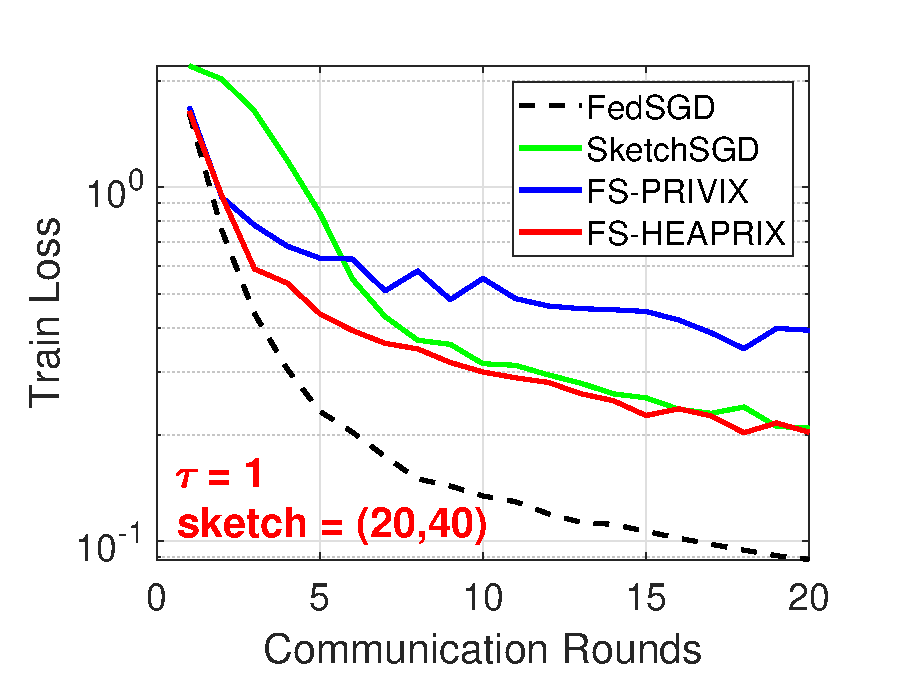
\includegraphics[width=3in]{MNIST_figures/local1_sketch20_iid1_train_loss.eps}
		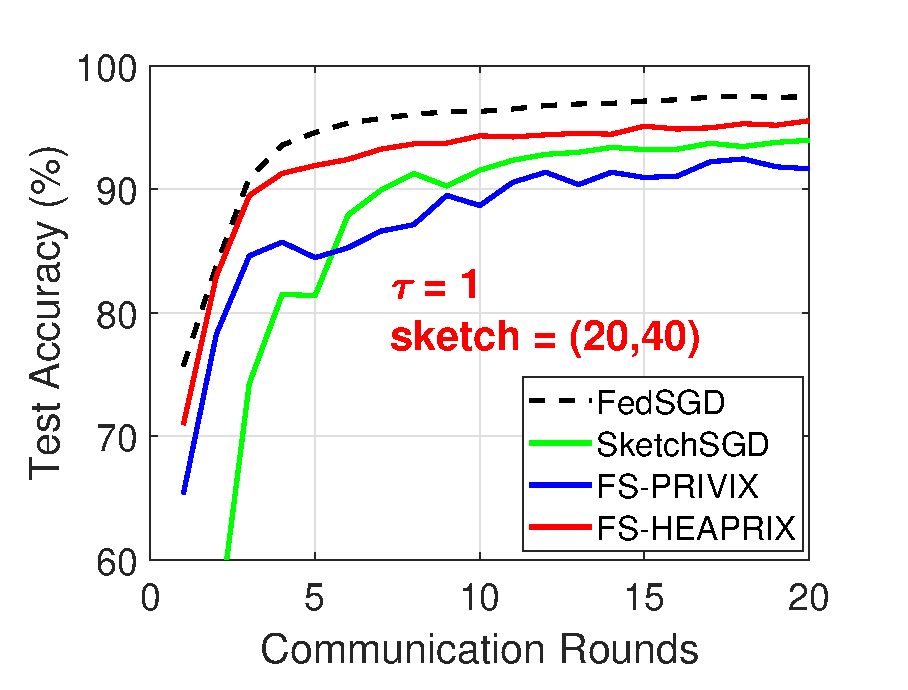
\includegraphics[width=3in]{MNIST_figures/local1_sketch20_iid1_test_acc.eps}
		}
		\mbox{
		\includegraphics[width=3in]{MNIST_figures/local1_sketch50_iid1_train_loss.eps}
		\includegraphics[width=3in]{MNIST_figures/local1_sketch50_iid1_test_acc.eps}
		}
	\end{center}
	\caption{The comparison of four algorithms on LeNet CNN architecture.}
    \label{fig:MNIST-tau1}
\end{figure}

\begin{figure}[h]
	\begin{center}
		\mbox{			    \includegraphics[width=1.6in]{MNIST_figures/local2_sketch20_iid1_train_loss.eps}
		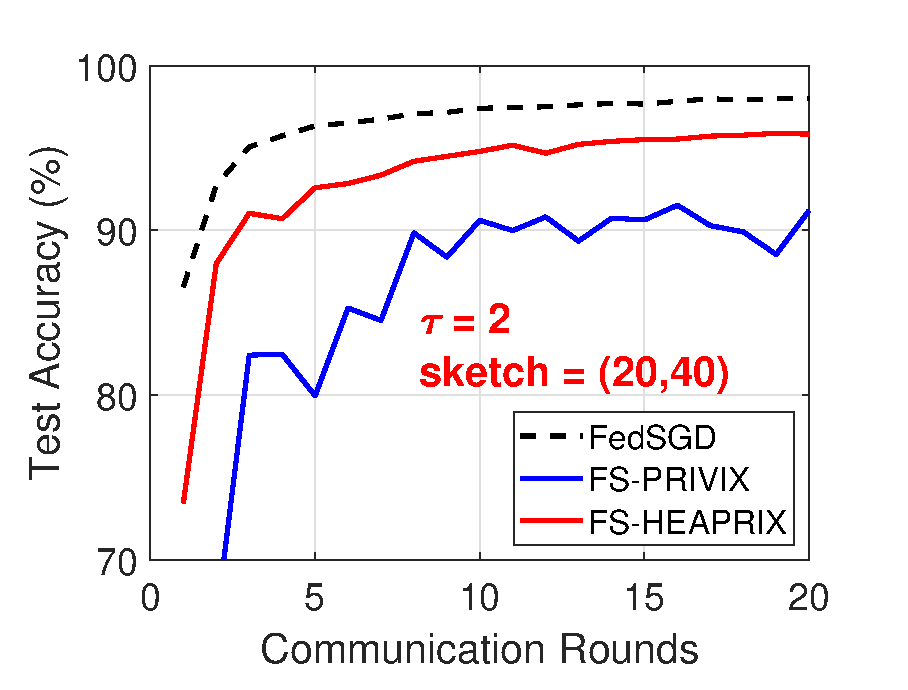
\includegraphics[width=1.6in]{MNIST_figures/local2_sketch20_iid1_test_acc.eps}
		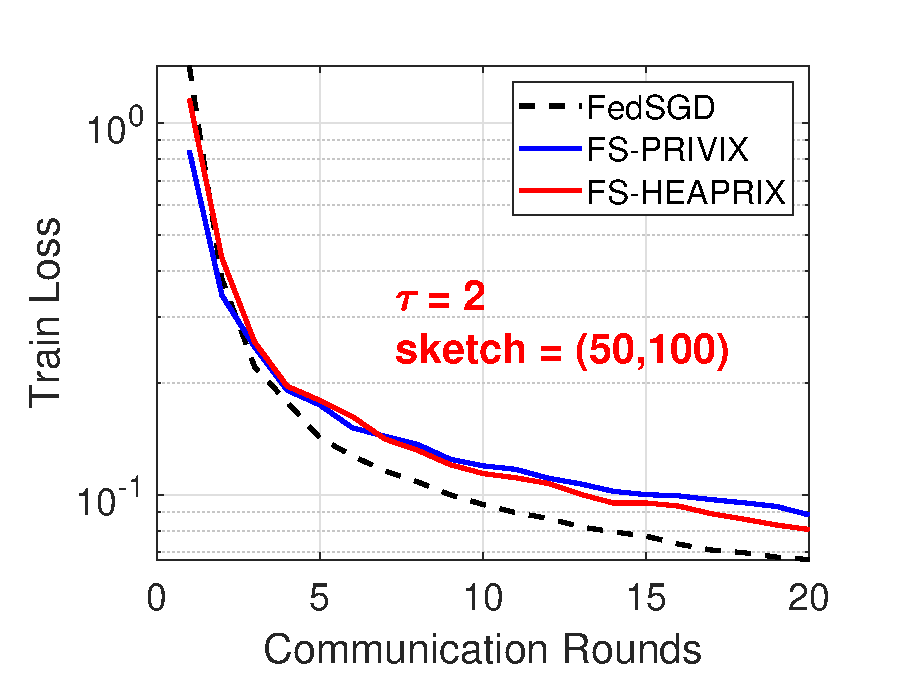
\includegraphics[width=1.6in]{MNIST_figures/local2_sketch50_iid1_train_loss.eps}
		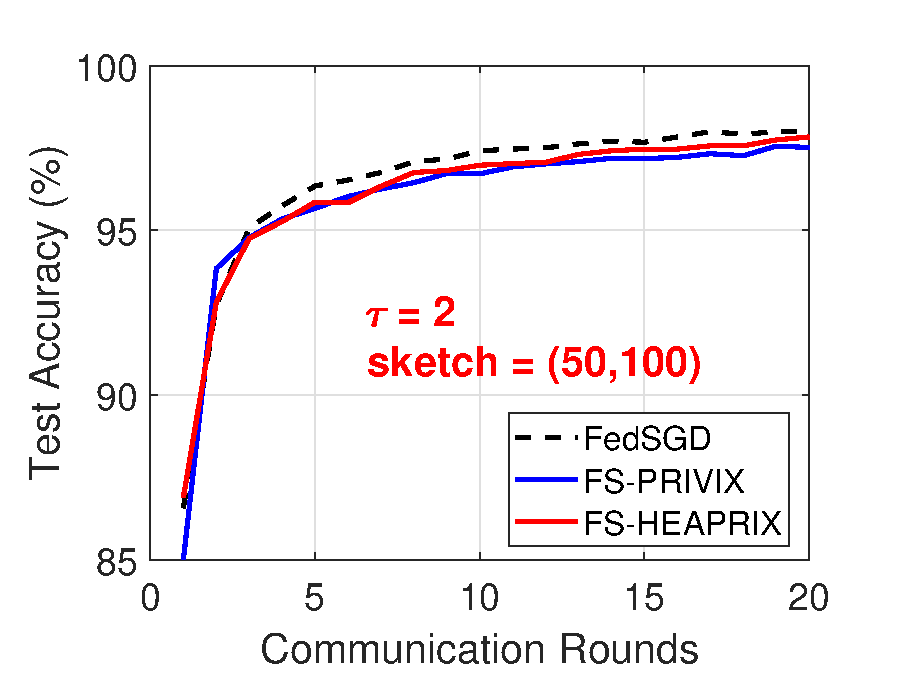
\includegraphics[width=1.6in]{MNIST_figures/local2_sketch50_iid1_test_acc.eps}
		}
		
		\mbox{			    \includegraphics[width=1.6in]{MNIST_figures/local5_sketch20_iid1_train_loss.eps}
		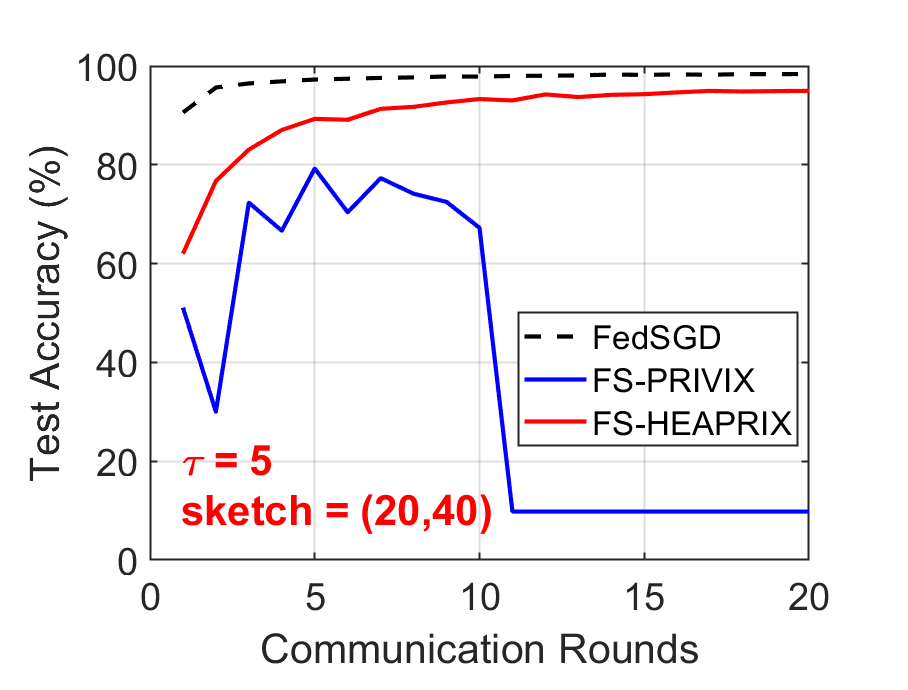
\includegraphics[width=1.6in]{MNIST_figures/local5_sketch20_iid1_test_acc.eps}
		\includegraphics[width=1.6in]{MNIST_figures/local5_sketch50_iid1_train_loss.eps}
		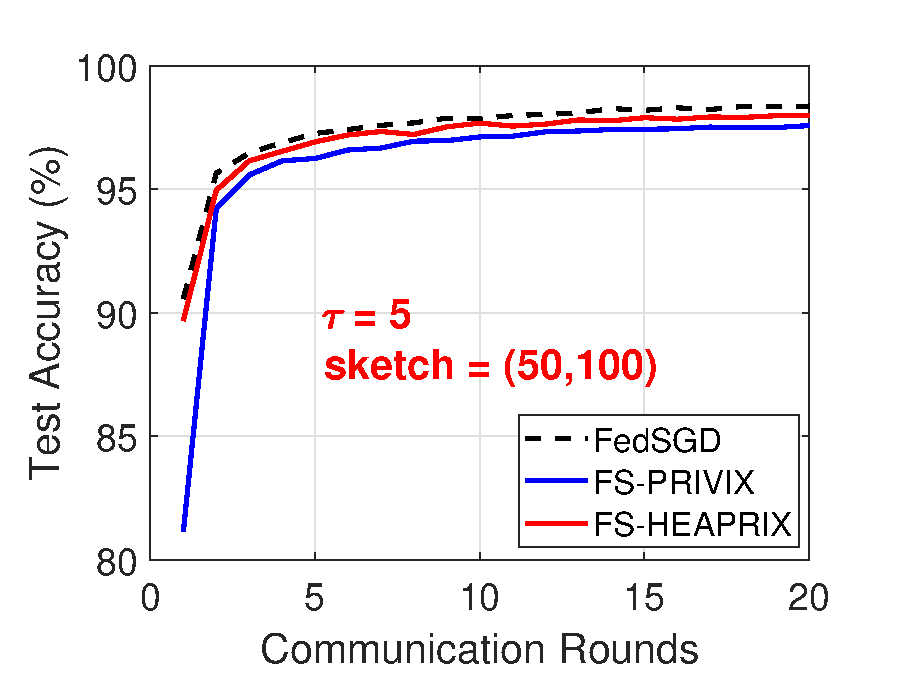
\includegraphics[width=1.6in]{MNIST_figures/local5_sketch50_iid1_test_acc.eps}
		}
	\end{center}
	\caption{Comparison of FedSGD, FS-PRIVIX and FS-HEAPRIX on LeNet CNN architecture, with number of local updates being 2 and 5.}
    \label{fig:MNIST-tau2,tau5}
\end{figure}


\textbf{Homogeneous case.} In Figure \ref{fig:MNIST-tau1} we provide the training loss and test accuracy of four algorithms with $\tau=1$ (since SketchSGD requires single local update per round). We also test different sizes of sketching matrix, $(t,k)=(20,40)$ and $(50,100)$. Note that these two choices of sketch size correspond to a $75\times$ and $12\times$ compression ratio, respectively. In general, as one would expect, higher compression ratio leads to worse learning performance. In both cases, FS-HEAPRIX performs the best in terms of both training objective and test accuracy. FS-PRIVIX is better when sketch size is large (i.e. when the estimation from sketches are more accurate), while SketchSGD performs better with small sketch size. 

The results for multiple local updates are given in Figure \ref{fig:MNIST-tau2,tau5}, where we set $\tau=2,5$. We see that FS-HEAPRIX is significantly better than FS-PRIVIX, either with small or large sketching matrix. In both cases, FS-HEAPRIX yields acceptable extra test error compared to FedSGD, especially taking the high compression ratio (e.g. $75\times$) into consideration. However, FS-PRIVIX performs poorly with small sketch size $(20,40)$, and even diverges with $\tau=5$. Another observation is that, the performance of FS-HEAPRIX improves with increasing number of local updates. That is, the proposed method is able to further reduce the communication cost by reducing the number of rounds required for communication. This is also consistent with our theoretical claims established in this paper.